%%%%%%%%%%%%%%%%%%%%%%%%%%%%%%%%%%%%%%%%%
% Short Sectioned Assignment
% LaTeX Template
% Version 1.0 (5/5/12)
%
% This template has been downloaded from:
% http://www.LaTeXTemplates.com
%
% Original author:
% Frits Wenneker (http://www.howtotex.com)
%
% License:
% CC BY-NC-SA 3.0 (http://creativecommons.org/licenses/by-nc-sa/3.0/)
%
%%%%%%%%%%%%%%%%%%%%%%%%%%%%%%%%%%%%%%%%%

%----------------------------------------------------------------------------------------
%	PACKAGES AND OTHER DOCUMENT CONFIGURATIONS
%----------------------------------------------------------------------------------------

\documentclass[paper=a4, fontsize=11pt]{scrartcl} % A4 paper and 11pt font size

\usepackage[T1]{fontenc} % Use 8-bit encoding that has 256 glyphs
\usepackage{fourier} % Use the Adobe Utopia font for the document - comment this line to return to the LaTeX default
\usepackage[english]{babel} % English language/hyphenation
\usepackage{amsmath,amsfonts,amsthm} % Math packages
\usepackage{sectsty} % Allows customizing section commands
\usepackage{graphicx}
\usepackage{fancyhdr} % Custom headers and footers
\usepackage{nicefrac}

\allsectionsfont{\fontsize{12}{15}\normalfont\bfseries} % Make all sections centered, the default font and small caps
\renewcommand\thesection{\arabic{section}}
\renewcommand\thesubsection{\alph{subsection}}

\pagestyle{fancyplain} % Makes all pages in the document conform to the custom headers and footers
\fancyhead{} % No page header - if you want one, create it in the same way as the footers below
\fancyfoot[L]{} % Empty left footer
\fancyfoot[C]{} % Empty center footer
\fancyfoot[R]{\thepage} % Page numbering for right footer
\renewcommand{\headrulewidth}{0pt} % Remove header underlines
\renewcommand{\footrulewidth}{0pt} % Remove footer underlines
\setlength{\headheight}{13.6pt} % Customize the height of the header

\numberwithin{equation}{section} % Number equations within sections (i.e. 1.1, 1.2, 2.1, 2.2 instead of 1, 2, 3, 4)
\numberwithin{figure}{section} % Number figures within sections (i.e. 1.1, 1.2, 2.1, 2.2 instead of 1, 2, 3, 4)
\numberwithin{table}{section} % Number tables within sections (i.e. 1.1, 1.2, 2.1, 2.2 instead of 1, 2, 3, 4)

\setlength\parindent{0pt} % Removes all indentation from paragraphs - comment this line for an assignment with lots of text

%----------------------------------------------------------------------------------------
%	TITLE SECTION
%----------------------------------------------------------------------------------------

\newcommand{\horrule}[1]{\rule{\linewidth}{#1}} % Create horizontal rule command with 1 argument of height

\title{	
\normalfont \normalsize 
\textsc{Fakultas Ilmu Komputer, Universitas Indonesia} \\ [8pt]  \textsc{CSC4602354  Natural Language Processing} \\ [8pt] 
\textsc {Worksheet 2 - Basic Text Processing, Language Model, \& POS Tagging}
%Your university, school and/or department name(s)
%\horrule{0.5pt} \\[0.4cm] % Thin top horizontal rule
%\huge Assignment Title \\ % The assignment title
%\horrule{2pt} \\[0.5cm] % Thick bottom horizontal rule
}

\author{	
	\small Yohanes Gultom \\
	\small 1506706345
	\and
	\small Arrianda Mardhika Adif \\
	\small 1306386882
} % Your name
\date{\normalsize\today} % Today's date or a custom date

\begin{document}

\maketitle % Print the title


\section{Heuristic rules untuk Sentence Splitter Bahasa Indonesia}

\begin{enumerate}	
\item Penggal kalimat menggunakan {\em delimiter} ". " (titik + spasi) dengan pengecualian ({\em exceptions}): 
\begin{itemize}	
	\item Gelar ({\em salutation} \& {\em degree}), contoh: "dr. ", "S.T. ", "MM" 
	\item Singkatan ({\em abbreviation}), contoh: "Jl. ", "No. ", "Kav. " 
\end{itemize}
Pengecualian dibutuhkan karena morfem tersebut terdiri dari ". " tetapi bukan merupakan akhir dari kalimat.
\item Penggal kalimat yang dipisahkan {\em newline}. Rule ini dibutuhkan jika karya sastra seperti pantun atau puisi yang tidak menggunakan titik untuk memisahkan kalimat.
\end{enumerate}

%------------------------------------------------

\section{Word Segmentation untuk Bahasa Indonesia}

Segmentasi kata ({\em word segmentation}) dalam bahasa Indonesia dapat dilakukan hanya dengan menggunakan {\em delimiter} berupa " " (spasi) karena kami tidak menemukan:
\begin{enumerate}
	\item Kata yang dipisahkan spasi atau
	\item Kata yang tidak dipisahkan spasi
\end{enumerate}

%\begin{align}
%A = 
%\begin{bmatrix}
%A_{11} & A_{21} \\
%A_{21} & A_{22}
%\end{bmatrix}
%\end{align}

%------------------------------------------------

\section{POS Tagging}

\subsection{Part of Speech Tagging manual}

\begin{enumerate}
	\item (Pawang, BD) (bisa, KR)\footnote{http://kbbi.web.id/bisa} (menaklukkan, KR) (ular, BD)
	\item (Anak, BD) (itu, XX) (digigit, KR) (ular, BD) (dan, XX) (keracunan, KR) (bisa, BD)
	\item (Ular, BD) (bisa, KR) (menyerang, KR) (pawang, BD)
	\item (Pawang, BD) (bisa, KR) (keracunan, KR) (bisa, BD) (ular, BD)
	\item (Bisa, BD) (ular, BD) (bisa, KR) (jadi, KR) (penawar, BD)
\end{enumerate}

\subsection{HMM FSA}
Hasil training HMM FSA dengan data 1-4:

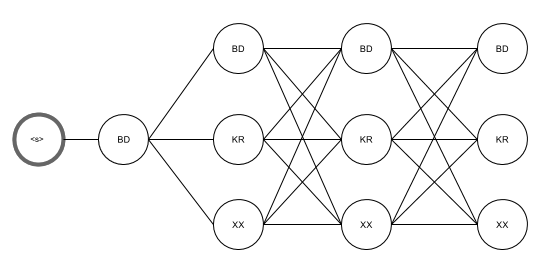
\includegraphics[scale=0.8]{hmm_fsa_pos_tagging_training}

Transition Probability \\
\begin{tabular}{ | l | c | c | c | c |}
\hline
From / To & BD & KR & XX \\ \hline
<s> & $\nicefrac{4}{4}$ & 0 & 0\\ \hline
BD & $\nicefrac{1}{6}$ & $\nicefrac{3}{6}$ & $\nicefrac{2}{6}$ \\ \hline
KR & $\nicefrac{5}{8}$ & $\nicefrac{3}{8}$ & 0 \\ \hline
XX & 0 & $\nicefrac{2}{2}$ & 0 \\ \hline
\end{tabular} \\ [8pt]

Emission Probability \\
\begin{tabular}{ | l | c | c | c | c | c | c | c | c | c | c |}
	\hline
	From / To & Pawang & Bisa & {\tiny Menaklukkan} & Ular & Anak & Itu & {\tiny Digigit} & Dan & {\tiny Keracunan} & {\tiny Menyerang} \\ \hline
	BD & $\nicefrac{3}{10}$ & $\nicefrac{2}{10}$ & 0 & $\nicefrac{4}{10}$ & $\nicefrac{1}{10}$ & 0 & 0 & 0 & 0 & 0 \\ \hline
	KR & 0 & $\nicefrac{3}{8}$ & $\nicefrac{1}{8}$ & 0 & 0 & 0 & $\nicefrac{1}{8}$ & 0 & $\nicefrac{2}{8}$ & $\nicefrac{1}{8}$ \\ \hline
	XX & 0 & 0 & 0 & 0 & 0 & $\nicefrac{1}{2}$ & 0 & $\nicefrac{1}{2}$ & 0 & 0 \\ \hline
\end{tabular}

\subsection{Testing Kalimat 5}

Dengan menggunakan algoritma Viterbi menggunakan informasi Transition dan Emission Probability:
\begin{enumerate}
	\item Bisa :
	\begin{itemize}
		\item \textbf{BD = P(BD|<s>) + P(bisa|BD) = 1 + $\nicefrac{2}{10}$ = 1.2}				
		\item KR = P(KR|<s>) + P(bisa|KR) = 0 + $\nicefrac{3}{8}$ = 0.375
		\item XX = P(XX|<s>) + P(bisa|XX) = 0 + 0 = 0				
	\end{itemize}
	\item Ular :
	\begin{itemize}
		\item \textbf{BD = P(BD|BD) + P(ular|BD) = $\nicefrac{1}{6}$ + $\nicefrac{4}{10}$ = 0.56}				
		\item KR = P(KR|BD) + P(ular|KR) = $\nicefrac{3}{6}$ + 0 = 0.5
		\item XX = P(XX|BD) + P(ular|XX) = $\nicefrac{2}{6}$ + 0 = 0.3				
	\end{itemize}
	\item Bisa :
	\begin{itemize}
		\item BD = P(BD|BD) + P(bisa|BD) = $\nicefrac{1}{6}$ + $\nicefrac{2}{10}$ = 0.36
		\item \textbf{KR = P(KR|BD) + P(bisa|KR) = $\nicefrac{3}{6}$ + $\nicefrac{3}{8}$ = 0.875}
		\item XX = P(XX|BD) + P(bisa|XX) = $\nicefrac{2}{6}$ + 0 = 0.3				
	\end{itemize}
	\item Jadi : 
	\begin{itemize}
		\item \textbf{BD = P(BD|KR) + P(jadi|BD) = $\nicefrac{5}{8}$ + 0 = 0.625}
		\item KR = P(KR|KR) + P(jadi|KR) = $\nicefrac{3}{8}$ + 0 = 0.375
		\item XX = P(XX|KR) + P(jadi|XX) = 0 + 0 = 0
	\end{itemize}
	\item Penawar : 
	\begin{itemize}
		\item BD = P(BD|BD) + P(penawar|BD) = $\nicefrac{1}{6}$ + 0 = 0.16
		\item \textbf{KR = P(KR|BD) + P(penawar|KR) = $\nicefrac{3}{6}$ + 0 = 0.5}
		\item XX = P(XX|BD) + P(penawar|XX) = $\nicefrac{2}{6}$ + 0 = 0.3
	\end{itemize}		
\end{enumerate}
HMM : (Bisa, BD) (ular, BD) (bisa, KR) (jadi, \textbf{BD}) (penawar, \textbf{KR}) \\
Manual : (Bisa, BD) (ular, BD) (bisa, KR) (jadi, KR) (penawar, BD) \\
Hasil tagging HMM hanya memiliki akurasi \textbf{60\%} dibanding dengan tagging manual.

\subsection{Penerapan Laplace Smoothing}

Transition Probability \\
\begin{tabular}{ | l | c | c | c | }
	\hline
	From / To & BD & KR & XX \\ \hline
	<s> & $\nicefrac{5}{7}$ & $\nicefrac{1}{7}$ & $\nicefrac{1}{7}$ \\ \hline
	BD & $\nicefrac{2}{9}$ & $\nicefrac{4}{9}$ & $\nicefrac{3}{9}$ \\ \hline
	KR & $\nicefrac{6}{11}$ & $\nicefrac{4}{11}$ & $\nicefrac{1}{11}$ \\ \hline
	XX & $\nicefrac{1}{5}$ & $\nicefrac{3}{5}$ & $\nicefrac{1}{5}$ \\ \hline
\end{tabular} \\ [8pt]

Emission Probability \\
\begin{tabular}{ | l | c | c | c | c | c | c | c | c | c | c | c |}
	\hline
	From / To & Pawang & Bisa & {\tiny Menaklukkan} & Ular & Anak & Itu & {\tiny Digigit} & Dan & {\tiny Keracunan} & {\tiny Menyerang} & {\tiny Kata Baru}\\ \hline
	BD & $\nicefrac{4}{21}$ & $\nicefrac{3}{21}$ & $\nicefrac{1}{21}$ & $\nicefrac{5}{21}$ & $\nicefrac{2}{21}$ & $\nicefrac{1}{21}$ & $\nicefrac{1}{21}$ & $\nicefrac{1}{21}$ & $\nicefrac{1}{21}$ & $\nicefrac{1}{21}$ & $\nicefrac{1}{21}$ \\ \hline
	KR & $\nicefrac{1}{19}$ & $\nicefrac{4}{19}$ & $\nicefrac{2}{19}$ & $\nicefrac{1}{19}$ & $\nicefrac{1}{19}$ & $\nicefrac{1}{19}$ & $\nicefrac{2}{19}$ & $\nicefrac{1}{19}$ & $\nicefrac{3}{19}$ & $\nicefrac{3}{19}$ & $\nicefrac{1}{19}$ \\ \hline
	XX & $\nicefrac{1}{13}$ & $\nicefrac{1}{13}$ & $\nicefrac{1}{13}$ & $\nicefrac{1}{13}$ & $\nicefrac{1}{13}$ & $\nicefrac{2}{13}$ & $\nicefrac{1}{13}$ & $\nicefrac{2}{13}$ & $\nicefrac{1}{13}$ & $\nicefrac{1}{13}$ & $\nicefrac{1}{13}$ \\ \hline
\end{tabular} \\ [8pt]

Virtebi
\begin{enumerate}
	\item Bisa :
	\begin{itemize}
		\item \textbf{BD = P(BD|<s>) + P(bisa|BD) = $\nicefrac{5}{7}$ + $\nicefrac{3}{21}$ = 0.85}				
		\item KR = P(KR|<s>) + P(bisa|KR) = $\nicefrac{1}{7}$ + $\nicefrac{4}{19}$ = 0.35
		\item XX = P(XX|<s>) + P(bisa|XX) = $\nicefrac{1}{7}$ + $\nicefrac{1}{13}$ = 0.21				
	\end{itemize}
	\item Ular :
	\begin{itemize}
		\item \textbf{BD = P(BD|BD) + P(ular|BD) = $\nicefrac{2}{9}$ + $\nicefrac{5}{21}$ = 0.46}				
		\item KR = P(KR|BD) + P(ular|KR) = $\nicefrac{4}{9}$ + $\nicefrac{1}{19}$ = 0.49
		\item XX = P(XX|BD) + P(ular|XX) = $\nicefrac{3}{9}$ + $\nicefrac{1}{13}$ = 0.41			
	\end{itemize}
	\item Bisa :
	\begin{itemize}
		\item BD = P(BD|BD) + P(bisa|BD) = $\nicefrac{2}{9}$ + $\nicefrac{3}{21}$ = 0.36
		\item \textbf{KR = P(KR|BD) + P(bisa|KR) = $\nicefrac{4}{9}$ + $\nicefrac{4}{19}$ = 0.65}
		\item XX = P(XX|BD) + P(bisa|XX) = $\nicefrac{3}{9}$ + $\nicefrac{1}{13}$ = 0.41				
	\end{itemize}
	\item Jadi : 
	\begin{itemize}
		\item \textbf{BD = P(BD|KR) + P(jadi|BD) = $\nicefrac{6}{11}$ + $\nicefrac{1}{21}$ = 0.59}
		\item KR = P(KR|KR) + P(jadi|KR) = $\nicefrac{4}{11}$ + $\nicefrac{1}{19}$ = 0.41
		\item XX = P(XX|KR) + P(jadi|XX) = $\nicefrac{1}{11}$ + $\nicefrac{1}{13}$ = 0.16
	\end{itemize}
	\item Penawar : 
	\begin{itemize}
		\item BD = P(BD|BD) + P(penawar|BD) = $\nicefrac{2}{9}$ + $\nicefrac{1}{21}$ = 0.26
		\item \textbf{KR = P(KR|BD) + P(penawar|KR) = $\nicefrac{4}{9}$ + $\nicefrac{1}{19}$ = 0.49}
		\item XX = P(XX|BD) + P(penawar|XX) = $\nicefrac{3}{9}$ + $\nicefrac{1}{13}$ = 0.41
	\end{itemize}		
\end{enumerate}
Hasil: (Bisa, BD) (ular, BD) (bisa, KR) (jadi, \textbf{BD}) (penawar, \textbf{KR})
HMM dengan Laplace Smoothing memberikan \textbf{hasil dan akurasi yang sama yaitu 60\%}

\subsection{Penerapan Laplace Smoothing pada Unigram dan Trigram}

Unigram Transition Probability \\
\begin{tabular}{ |c | c | c | c |}
	\hline
	BD & KR & XX \\ \hline
	$\nicefrac{11}{23}$ & $\nicefrac{9}{23}$ & $\nicefrac{3}{23}$ \\ \hline
\end{tabular} \\ [8pt]

Unigram Virtebi
\begin{enumerate}
	\item Bisa :
	\begin{itemize}
		\item \textbf{BD = P(BD) + P(bisa|BD) = $\nicefrac{11}{23}$ + $\nicefrac{3}{21}$ = 0.62}				
		\item KR = P(KR) + P(bisa|KR) = $\nicefrac{9}{23}$ + $\nicefrac{4}{19}$ = 0.6
		\item XX = P(XX) + P(bisa|XX) = $\nicefrac{3}{23}$ + $\nicefrac{1}{13}$ = 0.2				
	\end{itemize}
	\item Ular :
	\begin{itemize}
		\item \textbf{BD = P(BD) + P(ular|BD) = $\nicefrac{11}{23}$ + $\nicefrac{5}{21}$ = 0.71}				
		\item KR = P(KR) + P(ular|KR) = $\nicefrac{9}{23}$ + $\nicefrac{1}{19}$ = 0.44
		\item XX = P(XX) + P(ular|XX) = $\nicefrac{3}{23}$ + $\nicefrac{1}{13}$ = 0.2			
	\end{itemize}
	\item Bisa :
	\begin{itemize}
		\item \textbf{BD = P(BD) + P(bisa|BD) = $\nicefrac{11}{23}$ + $\nicefrac{3}{21}$ = 0.62}
		\item KR = P(KR) + P(bisa|KR) = $\nicefrac{9}{23}$ + $\nicefrac{4}{19}$ = 0.60
		\item XX = P(XX) + P(bisa|XX) = $\nicefrac{3}{23}$ + $\nicefrac{1}{13}$ = 0.34				
	\end{itemize}
	\item Jadi : 
	\begin{itemize}
		\item \textbf{BD = P(BD) + P(jadi|BD) = $\nicefrac{11}{23}$ + $\nicefrac{1}{21}$ = 0.52}
		\item KR = P(KR) + P(jadi|KR) = $\nicefrac{9}{23}$ + $\nicefrac{1}{19}$ = 0.44
		\item XX = P(XX) + P(jadi|XX) = $\nicefrac{3}{23}$ + $\nicefrac{1}{13}$ = 0.2
	\end{itemize}
	\item Penawar : 
	\begin{itemize}
		\item \textbf{BD = P(BD) + P(penawar|BD) = $\nicefrac{11}{23}$ + $\nicefrac{1}{21}$ = 0.52}
		\item KR = P(KR) + P(penawar|KR) = $\nicefrac{9}{23}$ + $\nicefrac{1}{19}$ = 0.44
		\item XX = P(XX) + P(penawar|XX) = $\nicefrac{3}{23}$ + $\nicefrac{1}{13}$ = 0.2
	\end{itemize}		
\end{enumerate}

Hasil: (Bisa, BD) (ular, BD) (bisa, \textbf{BD}) (jadi, \textbf{BD}) (penawar, BD) \\
Hasil Unigram Laplace memberikan \textbf{hasil berbeda tapi dengan akurasi yang sama} dengan Bigram yaitu \textbf{60\%} \\

Trigram Transition Probability \\
\begin{tabular}{ | l | c | c | c |}
	\hline
	From / To & BD & KR & XX \\ \hline
	<s> <s> & $\nicefrac{5}{7}$ & $\nicefrac{1}{7}$ & $\nicefrac{1}{7}$ \\ \hline
	<s> BD & $\nicefrac{1}{7}$ & $\nicefrac{4}{7}$ & $\nicefrac{2}{7}$ \\ \hline
	<s> KR & $\nicefrac{1}{3}$ & $\nicefrac{1}{3}$ & $\nicefrac{1}{3}$ \\ \hline
	<s> XX & $\nicefrac{1}{3}$ & $\nicefrac{1}{3}$ & $\nicefrac{1}{3}$ \\ \hline
	BD BD & $\nicefrac{1}{4}$ & $\nicefrac{1}{4}$ & $\nicefrac{1}{4}$ \\ \hline
	BD KR & $\nicefrac{1}{6}$ & $\nicefrac{4}{6}$ & $\nicefrac{1}{6}$ \\ \hline
	BD XX & $\nicefrac{1}{5}$ & $\nicefrac{3}{5}$ & $\nicefrac{1}{5}$ \\ \hline	
	KR BD & $\nicefrac{2}{5}$ & $\nicefrac{1}{5}$ & $\nicefrac{2}{5}$ \\ \hline
	KR KR & $\nicefrac{4}{6}$ & $\nicefrac{1}{6}$ & $\nicefrac{1}{6}$ \\ \hline
	KR XX & $\nicefrac{1}{3}$ & $\nicefrac{1}{3}$ & $\nicefrac{1}{3}$ \\ \hline	
	XX BD & $\nicefrac{1}{3}$ & $\nicefrac{1}{3}$ & $\nicefrac{1}{3}$ \\ \hline
	XX KR & $\nicefrac{3}{5}$ & $\nicefrac{1}{5}$ & $\nicefrac{1}{5}$ \\ \hline
	XX XX & $\nicefrac{1}{3}$ & $\nicefrac{1}{3}$ & $\nicefrac{1}{3}$ \\ \hline		
\end{tabular} \\ [8pt]

Virtebi
\begin{enumerate}
	\item Bisa :
	\begin{itemize}
		\item \textbf{BD = P(BD|<s><s>) + P(bisa|BD) = $\nicefrac{5}{7}$ + $\nicefrac{3}{21}$ = 0.85}				
		\item KR = P(KR|<s><s>) + P(bisa|KR) = $\nicefrac{1}{7}$ + $\nicefrac{4}{19}$ = 0.35
		\item XX = P(XX|<s><s>) + P(bisa|XX) = $\nicefrac{1}{7}$ + $\nicefrac{1}{13}$ = 0.21				
	\end{itemize}
	\item Ular :
	\begin{itemize}
		\item BD = P(BD|<s>BD) + P(ular|BD) = $\nicefrac{1}{7}$ + $\nicefrac{5}{21}$ = 0.38
		\item KR = \textbf{P(KR|<s>BD) + P(ular|KR) = $\nicefrac{4}{7}$ + $\nicefrac{1}{19}$ = 0.62}
		\item XX = P(XX|<s>BD) + P(ular|XX) = $\nicefrac{2}{7}$ + $\nicefrac{1}{13}$ = 0.36	
	\end{itemize}
	\item Bisa :
	\begin{itemize}
		\item BD = P(BD|BD KR) + P(bisa|BD) = $\nicefrac{1}{6}$ + $\nicefrac{3}{21}$ = 0.30
		\item \textbf{KR = P(KR|BD KR) + P(bisa|KR) = $\nicefrac{4}{6}$ + $\nicefrac{4}{19}$ = 0.87}
		\item XX = P(XX|BD KR) + P(bisa|XX) = $\nicefrac{1}{6}$ + $\nicefrac{1}{13}$ = 0.24				
	\end{itemize}
	\item Jadi : 
	\begin{itemize}
		\item \textbf{BD = P(BD|KR KR) + P(jadi|BD) = $\nicefrac{4}{6}$ + $\nicefrac{1}{21}$ = 0.71}
		\item KR = P(KR|KR KR) + P(jadi|KR) = $\nicefrac{1}{6}$ + $\nicefrac{1}{19}$ = 0.21
		\item XX = P(XX|KR KR) + P(jadi|XX) = $\nicefrac{1}{6}$ + $\nicefrac{1}{13}$ = 0.24
	\end{itemize}
	\item Penawar : 
	\begin{itemize}
		\item BD = P(BD|KR BD) + P(penawar|BD) = $\nicefrac{2}{5}$ + $\nicefrac{1}{21}$ = 0.44
		\item KR = P(KR|KR BD) + P(penawar|KR) = $\nicefrac{1}{5}$ + $\nicefrac{1}{19}$ = 0.25
		\textbf{\item XX = P(XX|KR BD) + P(penawar|XX) = $\nicefrac{2}{5}$ + $\nicefrac{1}{13}$ = 0.47}
	\end{itemize}		
\end{enumerate}

Hasil: (Bisa, BD) (ular, \textbf{KR}) (bisa, KR) (jadi, \textbf{BD}) (penawar, \textbf{BD}) \\
Hasil Trigram Laplace memberikan \textbf{hasil berbeda dan dengan akurasi yang lebih buruk} dibanding Bigram yaitu \textbf{40\%}\\

\subsection{HMM Bigram dengan modifikasi data}

Training data
\begin{enumerate}
	\item (Pawang, BD) (bisa, KR)\footnote{http://kbbi.web.id/bisa} (menaklukkan, KR) (ular, BD)
	\item (Anak, BD) (itu, XX) (digigit, KR) (ular, BD) (dan, XX) (keracunan, KR) (bisa, BD)	
	\item (Bisa, BD) (ular, BD) (bisa, KR) (jadi, KR) (penawar, BD)
\end{enumerate}

Transition Probability \\
\begin{tabular}{ | l | c | c | c | c |}
	\hline
	From / To & BD & KR & XX \\ \hline
	<s> & $\nicefrac{3}{3}$ & 0 & 0 \\ \hline
	BD & $\nicefrac{1}{5}$ & $\nicefrac{2}{5}$ & $\nicefrac{2}{5}$ \\ \hline
	KR & $\nicefrac{4}{6}$ & $\nicefrac{2}{6}$ & 0 \\ \hline
	XX & 0 & $\nicefrac{2}{2}$ & 0 \\ \hline
\end{tabular} \\ [8pt]

Emission Probability \\
\begin{tabular}{ | l | c | c | c | c | c | c | c | c | c | c | c |}
	\hline
	From / To & Pawang & Bisa & {\tiny Menaklukkan} & Ular & Anak & Itu & {\tiny Digigit} & Dan & {\tiny Keracunan} & {\tiny Jadi} & {\tiny Penawar} \\ \hline
	BD & $\nicefrac{1}{8}$ & $\nicefrac{2}{8}$ & 0 & $\nicefrac{3}{8}$ & $\nicefrac{1}{8}$ & 0 & 0 & 0 & 0 & 0 & $\nicefrac{1}{8}$ \\ \hline
	KR & 0 & $\nicefrac{2}{6}$ & $\nicefrac{1}{6}$ & 0 & 0 & 0 & $\nicefrac{1}{6}$ & 0 & $\nicefrac{1}{6}$ & $\nicefrac{1}{6}$ & 0 \\ \hline
	XX & 0 & 0 & 0 & 0 & 0 & $\nicefrac{1}{2}$ & 0 & $\nicefrac{1}{2}$ & 0 & 0 & 0 \\ \hline
\end{tabular} \\ [8pt]

Testing data
\begin{enumerate}	
	\item (Ular, BD) (bisa, KR) (menyerang, KR) (pawang, BD)
	\item (Pawang, BD) (bisa, KR) (keracunan, KR) (bisa, BD) (ular, BD)
\end{enumerate}

Viterbi:
\begin{enumerate}
	\item Ular :
	\begin{itemize}
		\item \textbf{BD = P(BD|<s>) + P(ular|BD) = $\nicefrac{3}{3}$ + $\nicefrac{3}{8}$ = }				
		\item KR = P(KR|<s>) + P(ular|KR) = 0 + 0 = 0
		\item XX = P(XX|<s>) + P(ular|XX) = 0 + 0 = 0				
	\end{itemize}
	\item Bisa :
	\begin{itemize}
		\item BD = P(BD|BD) + P(bisa|BD) = $\nicefrac{1}{5}$ + $\nicefrac{2}{8}$ = 0.45
		\item \textbf{KR = P(KR|BD) + P(bisa|KR) = $\nicefrac{2}{5}$ + $\nicefrac{2}{6}$ = 0.73}
		\item XX = P(XX|BD) + P(bisa|XX) = $\nicefrac{2}{5}$ + 0 = 0.4				
	\end{itemize}
	\item Menyerang :
	\begin{itemize}
		\item \textbf{BD = P(BD|KR) + P(menyerang|BD) = $\nicefrac{4}{6}$ + 0 = 0.66}
		\item KR = P(KR|KR) + P(menyerang|KR) = $\nicefrac{2}{6}$ + 0 = 0.33
		\item XX = P(XX|KR) + P(menyerang|XX) = 0 + 0 = 0				
	\end{itemize}
	\item Pawang : 
	\begin{itemize}
		\item BD = P(BD|BD) + P(pawang|BD) = $\nicefrac{1}{5}$ + $\nicefrac{1}{8}$ = 0.325
		\item \textbf{KR = P(KR|BD) + P(pawang|KR) = $\nicefrac{2}{5}$ + 0 = 0.4}
		\item XX = P(XX|BD) + P(pawang|XX) = $\nicefrac{2}{5}$ + 0 = 0.4
	\end{itemize}		
\end{enumerate}

Hasil: (Ular, BD) (bisa, KR) (menyerang, \textbf{BD}) (pawang, \textbf{KR}) \\
Manual: (Ular, BD) (bisa, KR) (menyerang, KR) (pawang, BD) \\
Akurasi 50\%;

\begin{enumerate}
	\item Pawang :
	\begin{itemize}
		\item \textbf{BD = P(BD|<s>) + P(pawang|BD) = $\nicefrac{3}{3}$ + $\nicefrac{1}{8}$ = 1.125}				
		\item KR = P(KR|<s>) + P(pawang|KR) = 0 + 0 = 0
		\item XX = P(XX|<s>) + P(pawang|XX) = 0 + 0 = 0				
	\end{itemize}
	\item Bisa :
	\begin{itemize}
		\item BD = P(BD|BD) + P(bisa|BD) = $\nicefrac{1}{5}$ + $\nicefrac{2}{8}$ = 0.45
		\item \textbf{KR = P(KR|BD) + P(bisa|KR) = $\nicefrac{2}{5}$ + $\nicefrac{2}{6}$ = 0.73}
		\item XX = P(XX|BD) + P(bisa|XX) = $\nicefrac{2}{5}$ + 0 = 0.4				
	\end{itemize}
	\item Keracunan :
	\begin{itemize}
		\item \textbf{BD = P(BD|KR) + P(keracunan|BD) = $\nicefrac{4}{6}$ + 0 = 0.66}
		\item KR = P(KR|KR) + P(keracunan|KR) = $\nicefrac{2}{6}$ + $\nicefrac{1}{6}$ = 0.5
		\item XX = P(XX|KR) + P(keracunan|XX) = 0 + 0 = 0				
	\end{itemize}
	\item Bisa : 
	\begin{itemize}
		\item BD = P(BD|BD) + P(bisa|BD) = $\nicefrac{1}{5}$ + $\nicefrac{2}{8}$ = 0.45
		\item \textbf{KR = P(KR|BD) + P(bisa|KR) = $\nicefrac{2}{5}$ + $\nicefrac{2}{6}$ = 0.73}
		\item XX = P(XX|BD) + P(bisa|XX) = $\nicefrac{2}{5}$ + 0 = 0.4				
	\end{itemize}
	\item Ular :
	\begin{itemize}
		\item \textbf{BD = P(BD|KR) + P(ular|BD) = $\nicefrac{4}{6}$ + $\nicefrac{3}{8}$ = 1.04}
		\item KR = P(KR|KR) + P(ular|KR) = $\nicefrac{2}{6}$ + 0 = 0.3
		\item XX = P(XX|KR) + P(ular|XX) = 0 + 0 = 0				
	\end{itemize}	
\end{enumerate}

Hasil: (Pawang, BD) (bisa, KR) (keracunan, \textbf{BD}) (bisa, \textbf{KR}) (ular, BD) \\
Manual: (Pawang, BD) (bisa, KR) (keracunan, KR) (bisa, BD) (ular, BD) \\
Akurasi 60\% \\

\textbf{Rata-rata akurasi prediksi = (50 + 60) / 2 = 55\%} \\

\textbf{Kesimpulan}
\begin{enumerate}
	\item Hasil prediksi HMM dengan Viterbi sangat dipengaruhi oleh proporsi kemunculan kombinasi tag pada training data karena jumlah jenis tag jauh lebih sedikit dari jumlah tipe kata
	\item Nilai n-gram tidak selalu memberikan hasil yang lebih baik karena dapat mengamplifikasi kesalahan prediksi (dapat terjadi rantai error)
	\item Teknik smoothing dapat meningkatkan probabilitas prediksi kata baru tapi juga tetap dipengaruhi oleh faktor training data
\end{enumerate}	
\end{document}